%%%%%%%%%%%%%%%%%%%%%%%%%%%%%%%%%%%%%%%%%
% Short Sectioned Assignment
% LaTeX Template
% Version 1.0 (5/5/12)
%
% This template has been downloaded from:
% http://www.LaTeXTemplates.com
%
% Original author:
% Frits Wenneker (http://www.howtotex.com)
%
% License:
% CC BY-NC-SA 3.0 (http://creativecommons.org/licenses/by-nc-sa/3.0/)
%
%%%%%%%%%%%%%%%%%%%%%%%%%%%%%%%%%%%%%%%%%

%----------------------------------------------------------------------------------------
%	PACKAGES AND OTHER DOCUMENT CONFIGURATIONS
%----------------------------------------------------------------------------------------

\documentclass[paper=a4, fontsize=11pt]{scrartcl} % A4 paper and 11pt font size

\usepackage[T1]{fontenc} % Use 8-bit encoding that has 256 glyphs
%\usepackage{fourier} % Use the Adobe Utopia font for the document - comment this line to return to the LaTeX default
\usepackage[english]{babel} % English language/hyphenation
\usepackage{amsmath,amsfonts,amsthm} % Math packages

\usepackage{lipsum} % Used for inserting dummy 'Lorem ipsum' text into the template

\usepackage{sectsty} % Allows customizing section commands
\allsectionsfont{ \normalfont\scshape} % Make all sections centered, the default font and small caps

\usepackage{graphicx}
\usepackage{booktabs}
\usepackage[framed,numbered,autolinebreaks,useliterate]{mcode}

\usepackage{fancyhdr} % Custom headers and footers
\pagestyle{fancyplain} % Makes all pages in the document conform to the custom headers and footers
\fancyhead{} % No page header - if you want one, create it in the same way as the footers below
\fancyfoot[L]{} % Empty left footer
\fancyfoot[C]{} % Empty center footer
\fancyfoot[R]{\thepage} % Page numbering for right footer
\renewcommand{\headrulewidth}{0pt} % Remove header underlines
\renewcommand{\footrulewidth}{0pt} % Remove footer underlines
\setlength{\headheight}{12pt} % Customize the height of the header

\numberwithin{equation}{section} % Number equations within sections (i.e. 1.1, 1.2, 2.1, 2.2 instead of 1, 2, 3, 4)
\numberwithin{figure}{section} % Number figures within sections (i.e. 1.1, 1.2, 2.1, 2.2 instead of 1, 2, 3, 4)
\numberwithin{table}{section} % Number tables within sections (i.e. 1.1, 1.2, 2.1, 2.2 instead of 1, 2, 3, 4)

\setlength\parindent{0pt} % Removes all indentation from paragraphs - comment this line for an assignment with lots of text

%----------------------------------------------------------------------------------------
%	TITLE SECTION
%----------------------------------------------------------------------------------------

\newcommand{\horrule}[1]{\rule{\linewidth}{#1}} % Create horizontal rule command with 1 argument of height

\title{	
\normalfont \normalsize 
\textsc{APSC 1001, George Washington University} \\ [25pt] % Your university, school and/or department name(s)
\horrule{0.5pt} \\[0.4cm] % Thin top horizontal rule
\huge APSC 1001 Image Processing\\ % The assignment title
\horrule{2pt} \\[0.5cm] % Thick bottom horizontal rule
}

\author{\normalsize Randy Schur } % Your name

%\normalsize Week 1 Handout
\date{\normalsize \today } % Today's date or a custom date


\begin{document}

\maketitle % Print the title

\section{Introduction}
Image processing is a type of signal processing using an image as input. The output will either be another image, or statistics and parameters describing the image. Image processing is used by everyone - Photoshop and Instagram are two common examples, but engineers use it for tasks like medical diagnoses, object identification, and part inspection.\\

In order to capture an image, we use a camera. A camera is a sensor that can measure the intensity (and sometimes the wavelength) of light over an area. Often, this area is broken up into sections which we call pixels. A grayscale image has an intensity value for each pixel which determines how light or dark it is. Color images are often in RGB format, and have three intensity values at each pixel - one for red, green, and blue wavelengths.\\

In MATLAB, these intensities are stored in matrices. Each pixel has an intensity value ranging from 0 - 255, where 0 is completely dark and 255 is completely light. In a grayscale image, these correspond to black and white. To import an image, run the following commands: 
\lstinputlisting[firstline=8, lastline=11]{img_processing_in_class.m}

\section{Image Manipulation}
\subsection{Grayscale Images}
Notice that the image has a size of $n\times m\times 3$. Since this is an RGB (color) image, it has values for red, green, and blue at each pixel. We can do several manipulations with this image. The first is to turn it into grayscale, which may make it easier to run further image processing. Now, the image has size $n\times m$, because there is only a single intensity value at each pixel. The next step we are going to take is converting the image to black and white using a process called threshholding. Here, we go pixel by pixel through the grayscale image. If the pixel value is below a certain threshhold, we turn it black, otherwise we turn it white. Once reason for converting an image to black and white is that edges become easier to detect. 
\lstinputlisting[firstline=14, lastline=19]{img_processing_in_class.m}
\subsection{RGB Images}
Another manipulation that we can do is pulling out the red, green, and blue content of the image. Why might we do this? An analysis of the color content (frequency) of the image can give us a lot of information about the objects in the image. This strategy is particularly used in astronomy. In terms of aesthetics, this can allow us to modify only certain colors within an image. One way we can visualize this frequency content is to use a histogram, which tells us how many pixels there are that have a given intensity.\\

An RGB image can be thought of as three $n\times m$ matrices stacked up. Our strategy will be to take the first matrix from that stack and separate it out, which gives us all of the red intensities in the image. In order to display just the red parts of the image we will combine, or concatenate, the red intensities with zeros for the green and blue intensities. We can do the same for the other colors. 
\newpage
\lstinputlisting[firstline=21, lastline=46]{img_processing_in_class.m}

\subsection{Cropping}
Sometimes we want to look at only a section of the image rather than the entire image. Since images in MATLAB are stored as matrices, this is extremely simple to do! All we need is to take a subsection of the matrix, which is something we already have practice with using the : operator. 
\lstinputlisting[firstline=66, lastline=69]{img_processing_in_class.m}

\section{Filters}
Another type of image processing is called filtering. When you talk about adding an Instagram filter, what you are actually doing is manipulating the values for each pixel. When you watch a TV show and someone tells the computer geek to 'zoom in on that and sharpen it up,' they are again using image filtering. 

\subsection{Unsharpen Filter}
One of the most popular filters is called the Unsharpen filter, which does exactly the opposite of its name and sharpens up an image. \\

Let's assume that we have an image that is a little blurry. Either the camera was out of focus, or it was moved a bit while the image was taken. We are also going to assume that the distortion in the image is Gaussian, which means it follows a specific statistical distribution. This may or may not be an accurate assumption, but often in can be close to true.\\

The unsharpen filter takes the original image and blurs it using that Gaussian distribution. Then, we subtract the blurred image from the original image, in theory getting rid of some of the blur. Test out the code below to see if you get similar results.
\lstinputlisting[firstline=48, lastline=65]{img_processing_in_class.m}

\begin{figure}[h]
\centering
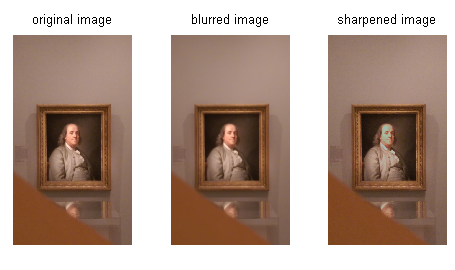
\includegraphics[scale=.95]{sharpened}
\end{figure}

It should be noted that applying filters to an image causes us to \textit{lose} information. However, we can often extract insights into the image at the expense of this lost information.

\section*{References}
[1] MATLAB Documentation, 2015.\\

[2] Image Processing Presentation, APSC 1001. Matthew Wilkins, 2014.

\end{document}